%% Background
\chapter{Background}
\label{chap:background}

\section{Font Selection}

Surprisingly little progress has been made in the past several decades on the issue of user font selection. When a user searches for a new font, almost every major word processor presents them with the same interface: a basic, linear list of typefaces with a few controls over additional parameters like size, weight, and underline. This interface—essentially the same interface as was used by the earliest multi-font word processors—offers users very little support or guidance when traversing the growing number of unique fonts available to them.

% from Designing the Xerox “Star” User Interface, Byte, issue 4, 1982
\begin{figure}[h]
    \centering
    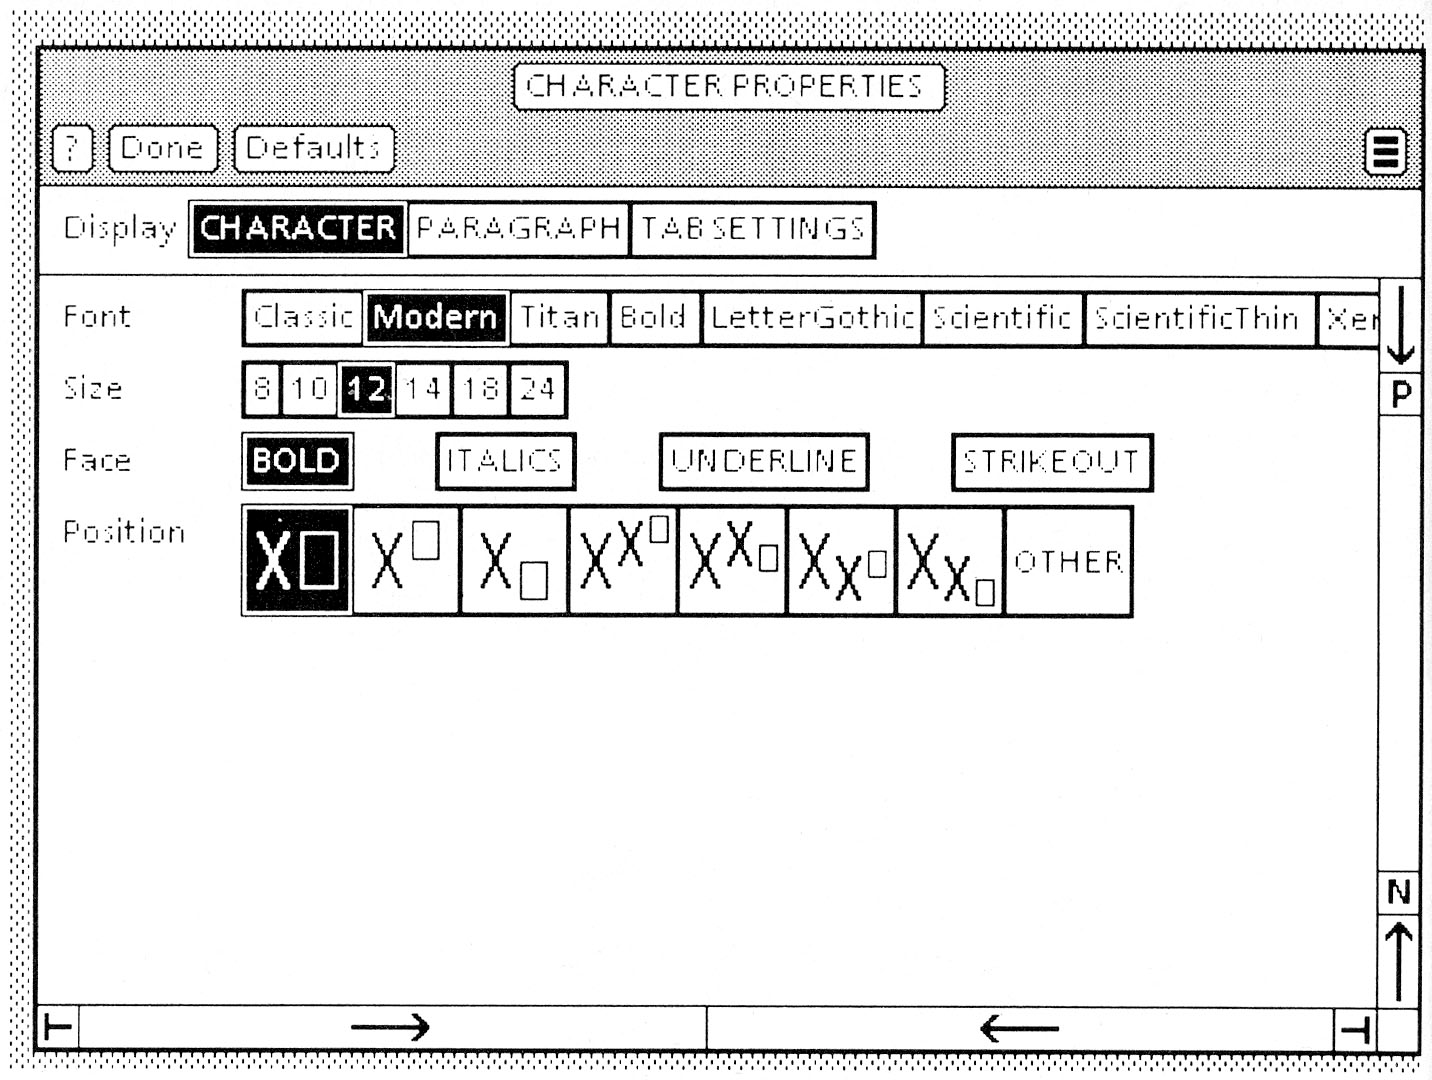
\includegraphics[width=.8\textwidth]{images/xerox-star.png}
    \caption{Font selection interface in Xerox Star (1981).}
    \label{fig:xerox-star}
\end{figure}

% own screenshots
\begin{figure}[h]
    \centering
    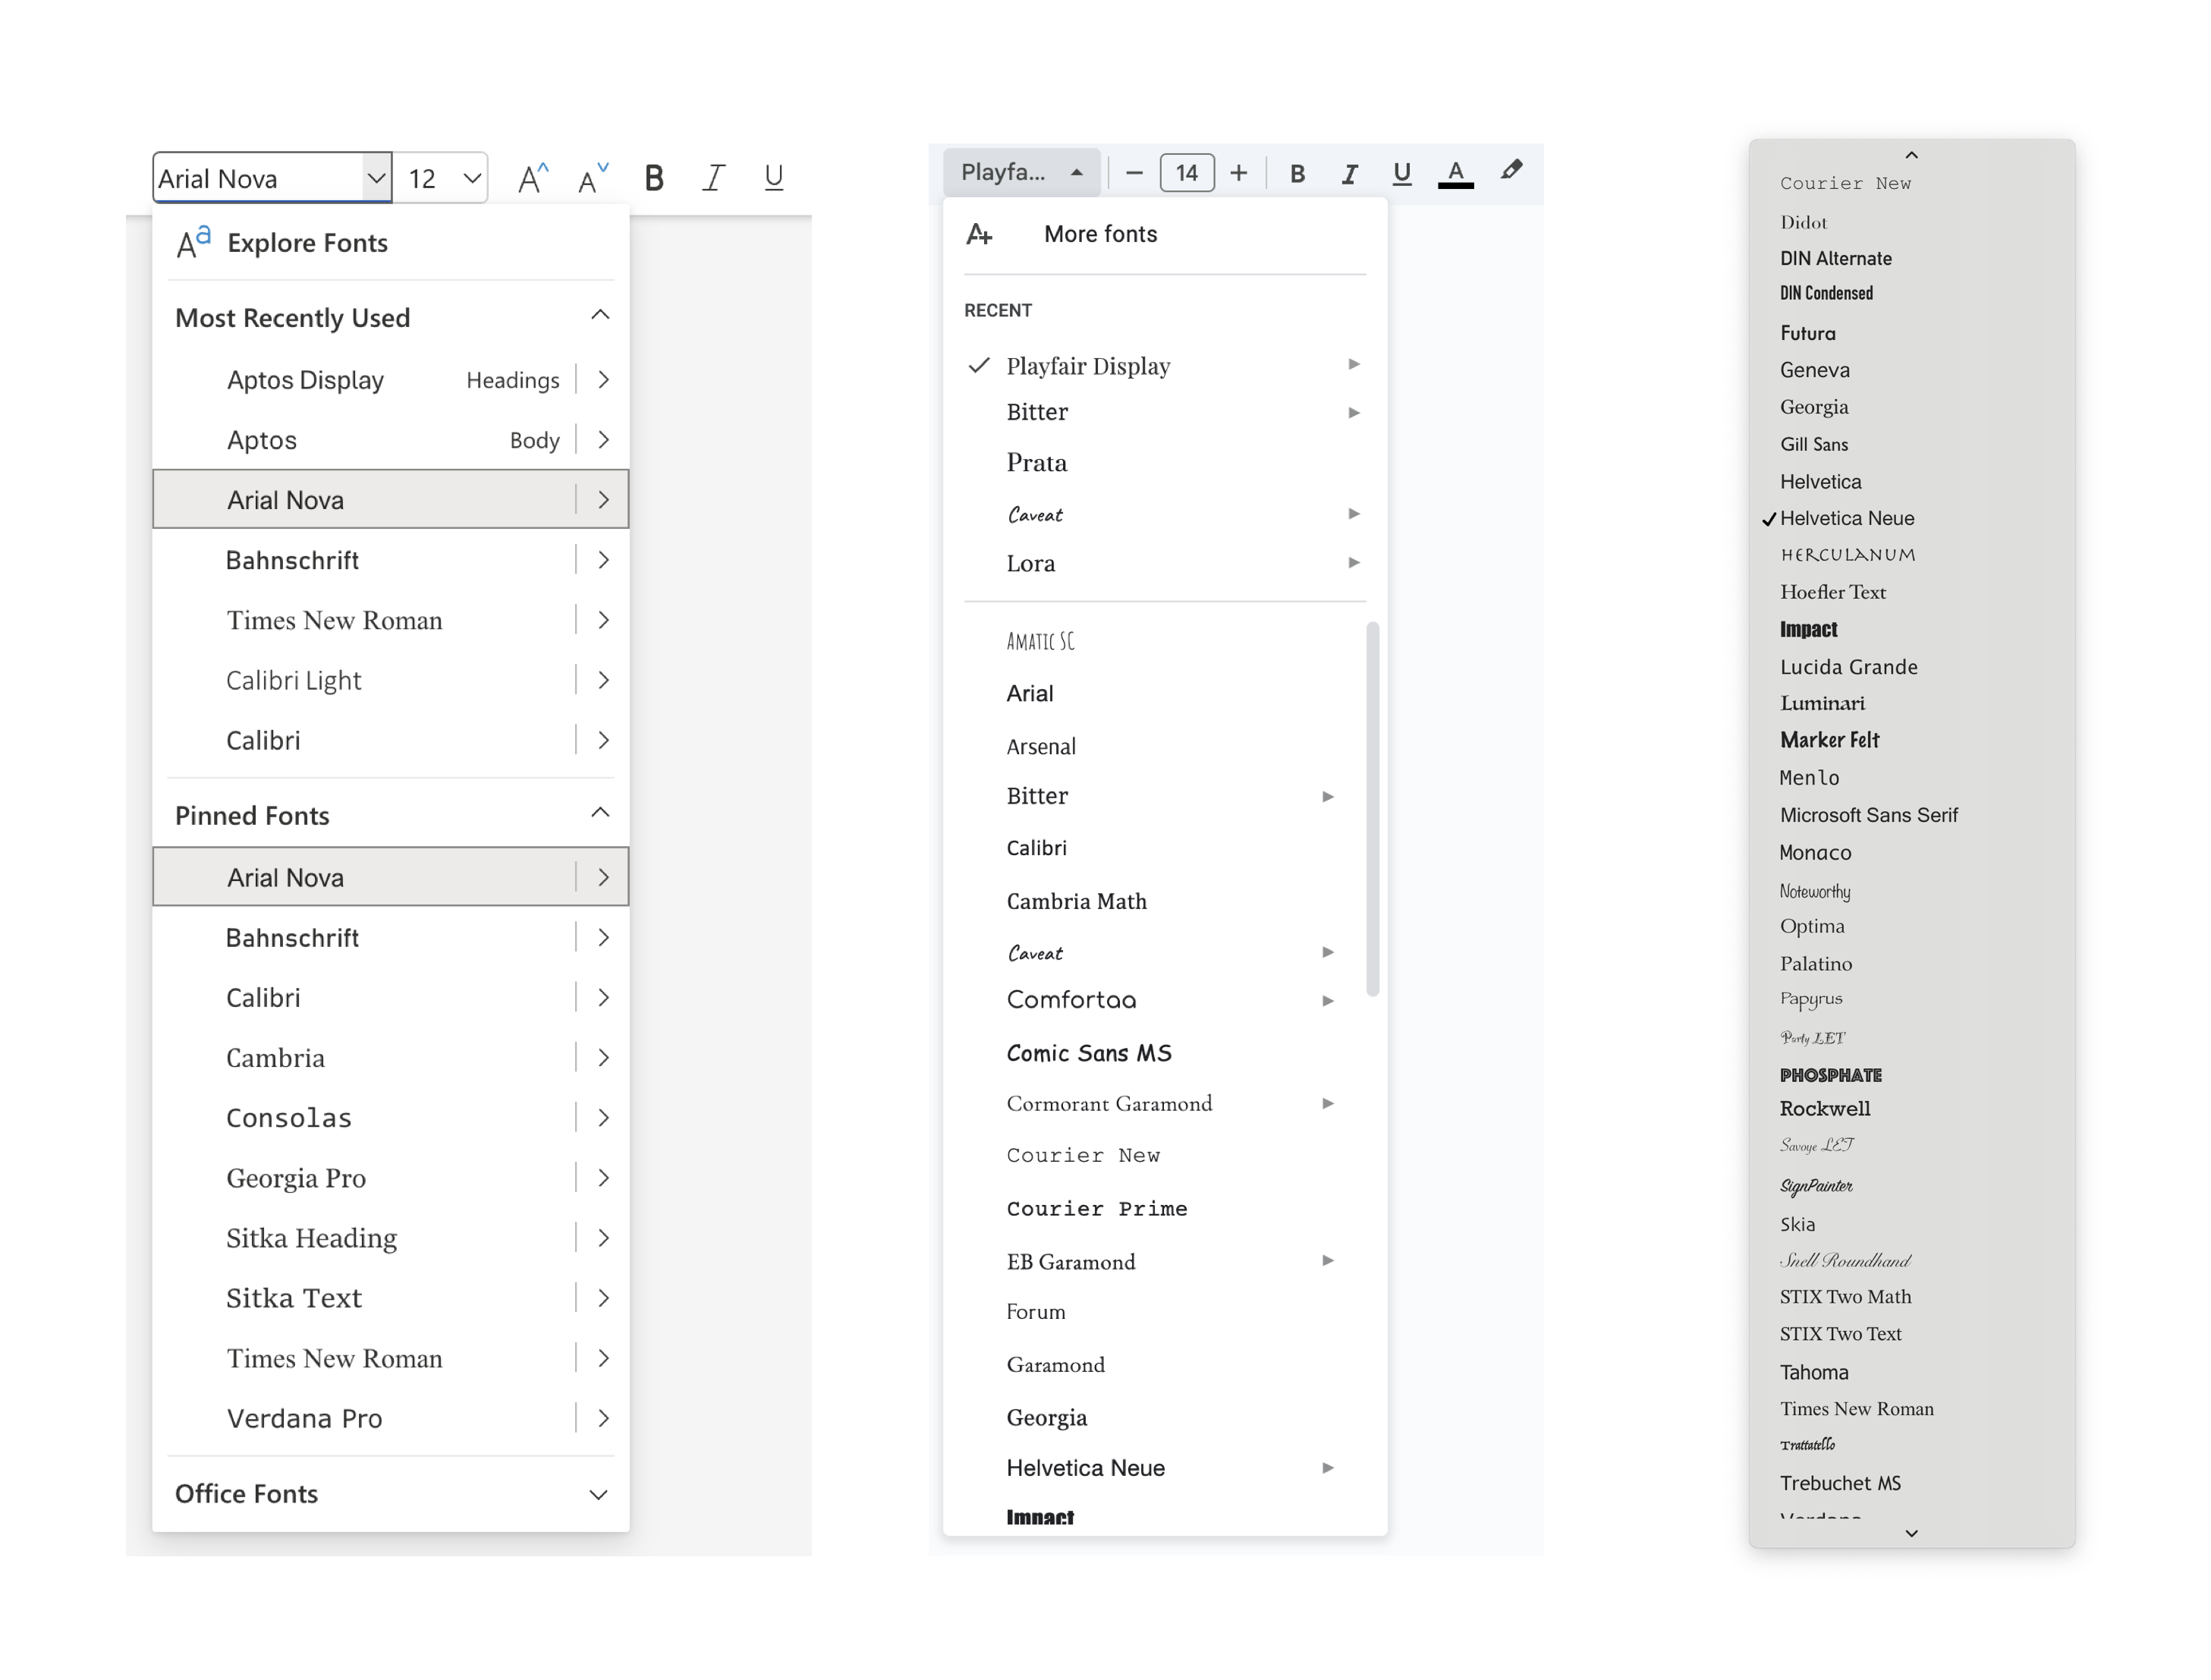
\includegraphics[width=1\textwidth]{images/font-selectors.png}
    \caption{Current font selection interfaces in Microsoft Word, Google Docs, and Apple Pages.}
    \label{fig:font-selectors}
\end{figure}

O'Donovan et al. list several reasons for the difficulty of developing font selection tools. The first issue is the sheer number of available fonts \cite{odonovan2014exploratory}. ``Most computers are now equipped with hundreds of fonts,'' they note, while online resources provide access to hundreds of thousands. Another issue is that there are not obvious ways to categorize fonts which correspond to a user's goal. While there exist broad categories like Serif, Sans Serif, and Handwritten, these must be manually designated on a per-font basis, and they do not necessarily categorize fonts along the lines which would be helpful for a user. A coffee shop owner deciding on a font for their shop's logo, for example, might not find the distinction between Serif and Sans Serif particularly useful, or know where to start in deciding between them. A graphic designer, who has studied design for years and has relevant experience, might feel confident in handling these decisions, but the typical user of a font selection tool does not have the tools, given the current font selector landscape, to make one of the most fundamental decisions to effective text-based graphical design. Finally, different users' goals in font selection vary. One user may be looking to match a particular font they found on a store sign, or to find a close match to a commercial font which is free to use. Another may be looking to match a particular mood, or choose a font that fits well with the rest of their document. A third may simply be exploring a large set of fonts like Adobe TypeKit or Google Fonts. O'Donovan et al. argues—and I agree—that current methods of font selection fall short on these issues and many more. Given the large number of fonts available to the modern user, a linear list of fonts is an  unrealistic and unhelpful tool.

Based on these issues, O'Donovan et al. presents three novel interfaces for font selection: one based on verbal attributes such as ``formal,'' ``friendly,'' or ``legible'' (Attribute Interface); another which clusters fonts hierarchically based on visual similarity (Group Interface); and a third, to be paired with the other two methods, which provides users with a list of similar font to the current selection (Search-By-Similarity). The researchers build these models on crowdsourced data collected through Amazon's Mechanical Turk with questions like ``Which of these two fonts is stronger?'', and they evaluated the interfaces using various design tasks on Mechanical Turk as well. Participants were three times more likely to succeed in a font-matching task, for example, using the Group Interface than the baseline font selector tool.

% own screenshots
\begin{figure}[h]
    \centering
    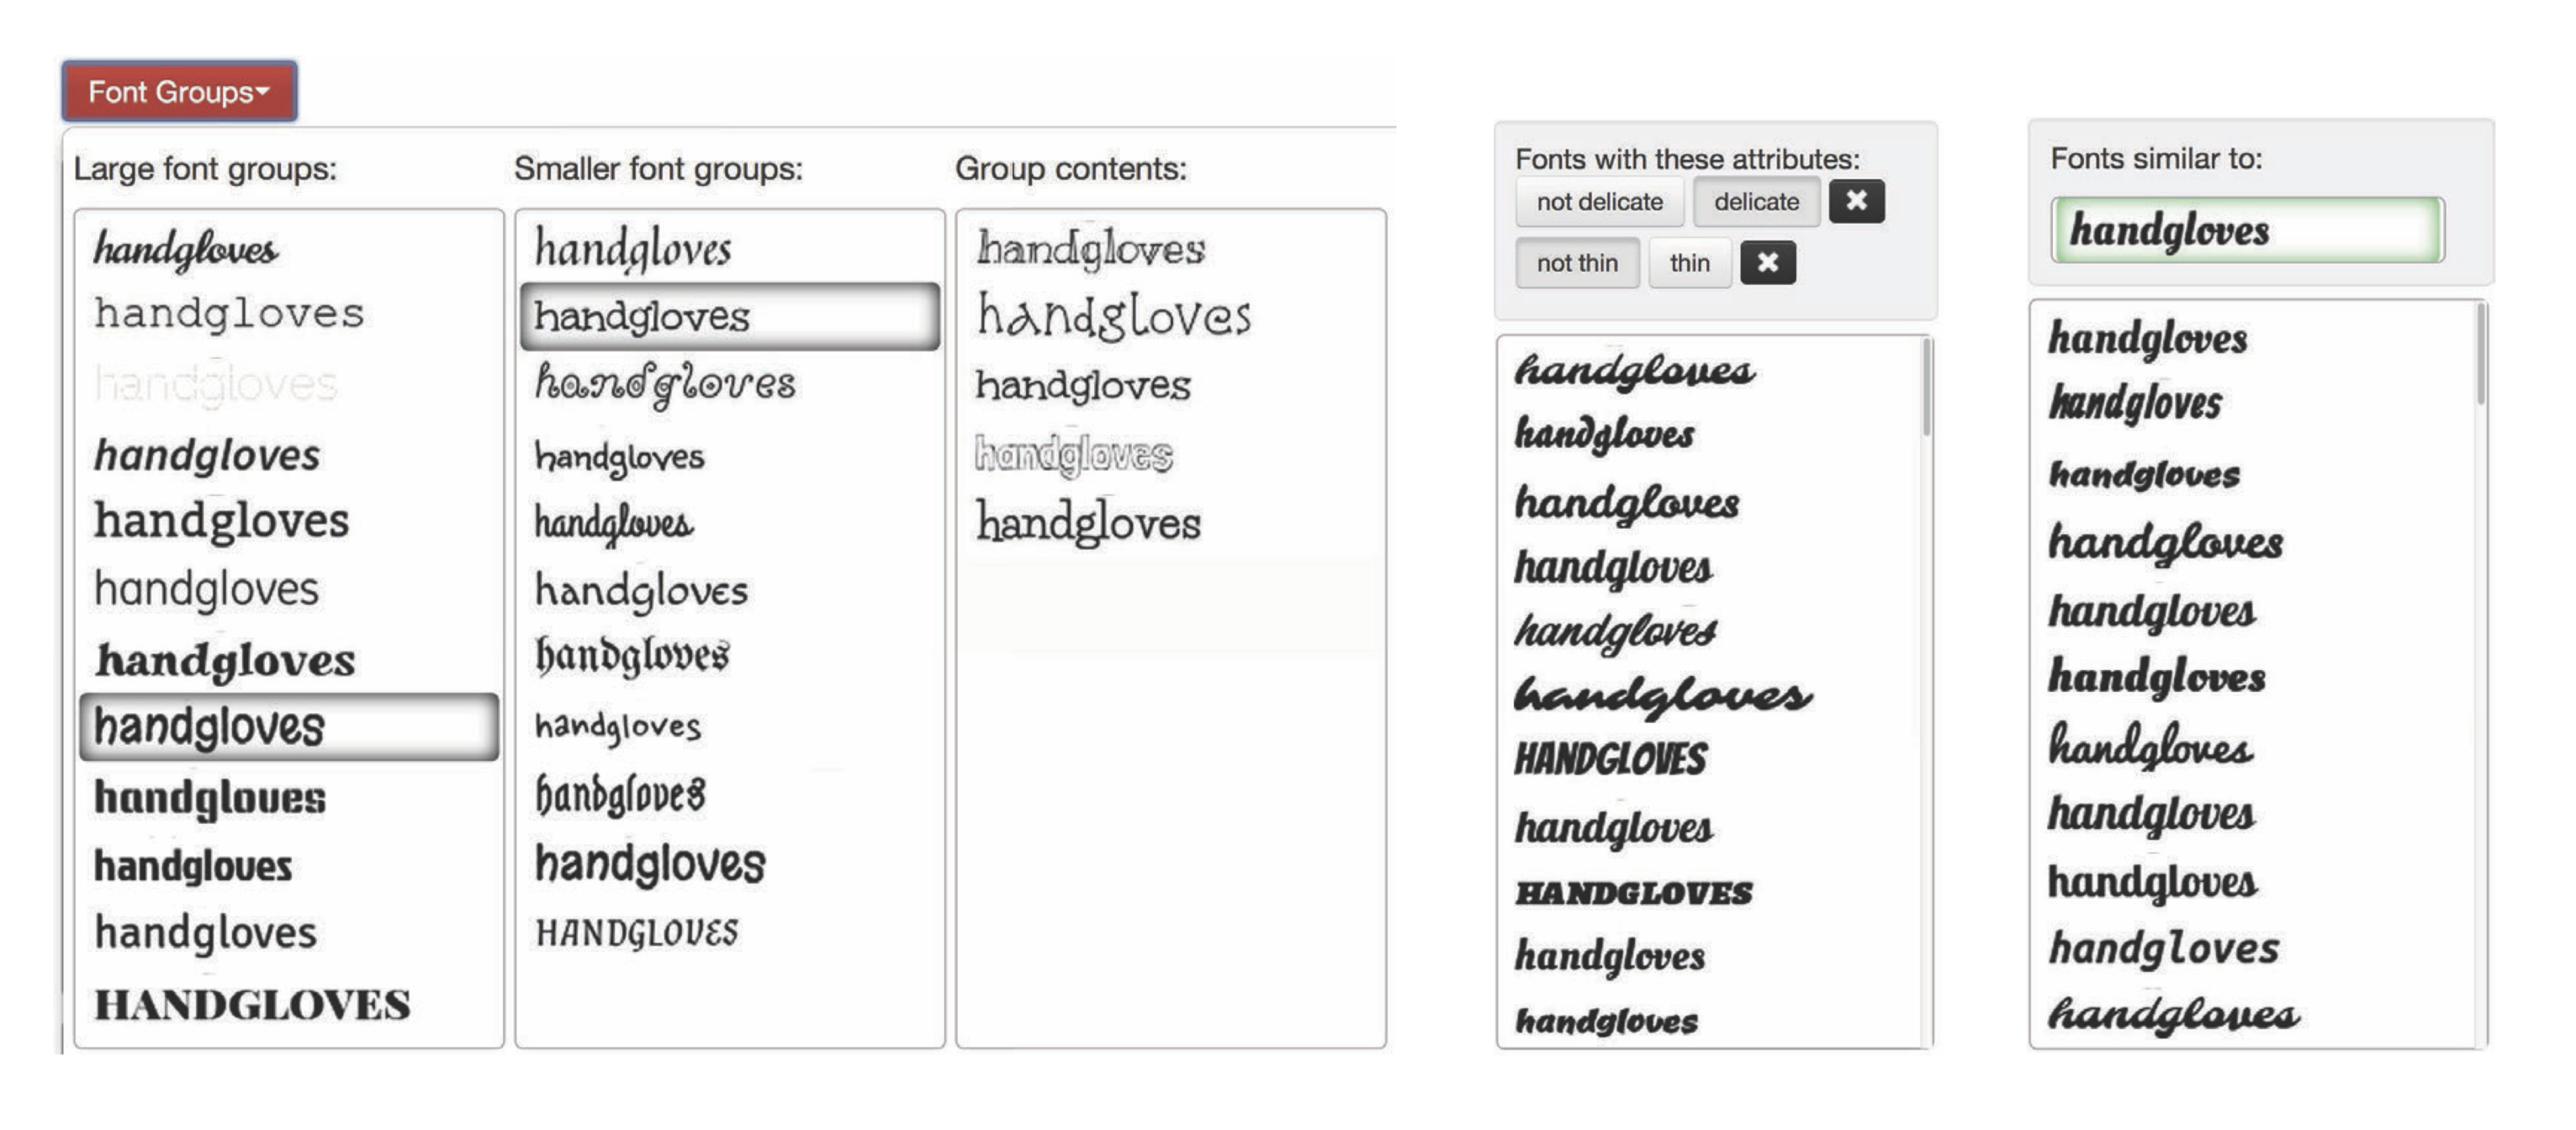
\includegraphics[width=1\textwidth]{images/odonovan-interfaces.png}
    \caption{Group Interface, Attribute Interface, and Search-By-Similarity selection tools from O'Donovan et al.}
    \label{fig:odonovan-interfaces}
\end{figure}